
%...........................................................
%
% Predicted number of events
%
%...........................................................

\section{Predicted number of events}
\label{app:events}

%In Tab.
%\ref{tab:nsk_nominal_no_osc_mulike_nu},~\ref{tab:nsk_nominal_osc_mulike_nu},
%\ref{tab:nsk_nominal_no_osc_mulike_nubar},~\ref{tab:nsk_nominal_osc_mulike_nubar},
%\ref{tab:nsk_nominal_no_osc_elike_nu},~\ref{tab:nsk_nominal_osc_elike_nu},
%\ref{tab:nsk_nominal_no_osc_elike_nubar} and~\ref{tab:nsk_nominal_osc_elike_nubar} 
%the predicted number of events is shown for 
%nominal MC, after applying the NA61/SHINE reweighting,
%after applying the NIWG tuning and 
%finally the BANFF tuning,
%both with oscillations consistent with ~\cref{tab:osc_params_joint}
%and without oscillations.
%
%
%\begin{table}
\begin{tabular} { | c ||c | c | c | c |  | }
\hline
                                                  & Nominal MC          & Flux-tuned MC       & BANFF prefit MC     & BANFF postfit MC     \\
                                                  &                     &                     & (flux + NIWG tune)  &                      \\ \hline  
Total                                             & 96.434              & 100.439             & 87.615              & 103.604              \\ \hline 
\hline 
$\nu_\mu$ CCQE                                    & 14.186              & 14.493              & 14.250              & 15.405               \\ \hline 
$\nu_\mu$ CC 1$\pi$                               & 4.792               & 5.019               & 5.019               & 3.666                \\ \hline 
$\nu_\mu$ CC coherent                             & 0.201               & 0.212               & 0.212               & 0.244                \\ \hline 
$\nu_\mu$ CC MEC                                  & 2.630               & 2.707               & 0.731               & 3.022                \\ \hline 
$\nu_\mu$ CC other                                & 1.198               & 1.307               & 1.307               & 1.393                \\ \hline 
$\nu_\mu$/$\nu_\tau$ NC 1$\pi^{+/-}$              & 0.495               & 0.523               & 0.523               & 0.340                \\ \hline 
$\nu_\mu$/$\nu_\tau$ NC 1$\pi^0$                  & 0.081               & 0.086               & 0.086               & 0.051                \\ \hline 
$\nu_\mu$/$\nu_\tau$ NC coherent                  & 0.001               & 0.001               & 0.001               & 0.001                \\ \hline 
$\nu_\mu$/$\nu_\tau$ NC other                     & 0.434               & 0.470               & 0.470               & 0.705                \\ \hline 
$\bar{\nu}_\mu$ CCQE                              & 53.188              & 55.834              & 50.852              & 57.962               \\ \hline 
$\bar{\nu}_\mu$ CC 1$\pi$                         & 7.506               & 7.658               & 7.658               & 6.746                \\ \hline 
$\bar{\nu}_\mu$ CC coherent                       & 2.409               & 2.515               & 2.515               & 3.082                \\ \hline 
$\bar{\nu}_\mu$ CC MEC                            & 7.382               & 7.699               & 2.079               & 9.037                \\ \hline 
$\bar{\nu}_\mu$ CC other                          & 0.914               & 0.891               & 0.891               & 1.005                \\ \hline 
$\bar{\nu}_\mu$/$\bar{\nu}_\tau$ NC 1$\pi^{+/-}$  & 0.571               & 0.581               & 0.581               & 0.381                \\ \hline 
$\bar{\nu}_\mu$/$\bar{\nu}_\tau$ NC 1$\pi^0$      & 0.081               & 0.082               & 0.082               & 0.048                \\ \hline 
$\bar{\nu}_\mu$/$\bar{\nu}_\tau$ NC coherent      & 0.006               & 0.006               & 0.006               & 0.007                \\ \hline 
$\bar{\nu}_\mu$/$\bar{\nu}_\tau$ NC other         & 0.265               & 0.260               & 0.260               & 0.410                \\ \hline 
$\nu_e$ CCQE                                      & 0.003               & 0.004               & 0.003               & 0.004                \\ \hline 
$\nu_e$ CC 1$\pi$                                 & 0.003               & 0.003               & 0.003               & 0.003                \\ \hline 
$\nu_e$ CC coherent                               & 0.000               & 0.000               & 0.000               & 0.000                \\ \hline 
$\nu_e$ CC MEC                                    & 0.001               & 0.001               & 0.000               & 0.001                \\ \hline 
$\nu_e$ CC other                                  & 0.001               & 0.001               & 0.001               & 0.001                \\ \hline 
$\nu_e$ NC 1$\pi^{+/-}$                           & 0.021               & 0.021               & 0.021               & 0.014                \\ \hline 
$\nu_e$ NC 1$\pi^0$                               & 0.003               & 0.004               & 0.004               & 0.002                \\ \hline 
$\nu_e$ NC coherent                               & 0.000               & 0.000               & 0.000               & 0.000                \\ \hline 
$\nu_e$ NC other                                  & 0.022               & 0.022               & 0.022               & 0.035                \\ \hline 
Osc. $\nu_e$ CCQE                                 & 0.000               & 0.000               & 0.000               & 0.000                \\ \hline 
Osc. $\nu_e$ CC 1$\pi$                            & 0.000               & 0.000               & 0.000               & 0.000                \\ \hline 
Osc. $\nu_e$ CC coherent                          & 0.000               & 0.000               & 0.000               & 0.000                \\ \hline 
Osc. $\nu_e$ CC MEC                               & 0.000               & 0.000               & 0.000               & 0.000                \\ \hline 
Osc. $\nu_e$ CC other                             & 0.000               & 0.000               & 0.000               & 0.000                \\ \hline 
$\bar{\nu}_e$ CCQE                                & 0.005               & 0.005               & 0.004               & 0.005                \\ \hline 
$\bar{\nu}_e$ CC 1$\pi$                           & 0.002               & 0.002               & 0.002               & 0.002                \\ \hline 
$\bar{\nu}_e$ CC coherent                         & 0.000               & 0.000               & 0.000               & 0.001                \\ \hline 
$\bar{\nu}_e$ CC MEC                              & 0.001               & 0.001               & 0.000               & 0.001                \\ \hline 
$\bar{\nu}_e$ CC other                            & 0.000               & 0.000               & 0.000               & 0.000                \\ \hline 
$\bar{\nu}_e$ NC 1$\pi^{+/-}$                     & 0.016               & 0.016               & 0.016               & 0.010                \\ \hline 
$\bar{\nu}_e$ NC 1$\pi^0$                         & 0.002               & 0.002               & 0.002               & 0.001                \\ \hline 
$\bar{\nu}_e$ NC coherent                         & 0.000               & 0.000               & 0.000               & 0.000                \\ \hline 
$\bar{\nu}_e$ NC other                            & 0.011               & 0.011               & 0.011               & 0.017                \\ \hline 
Osc. $\bar{\nu}_e$ CCQE                           & 0.000               & 0.000               & 0.000               & 0.000                \\ \hline 
Osc. $\bar{\nu}_e$ CC 1$\pi$                      & 0.000               & 0.000               & 0.000               & 0.000                \\ \hline 
Osc. $\bar{\nu}_e$ CC coherent                    & 0.000               & 0.000               & 0.000               & 0.000                \\ \hline 
Osc. $\bar{\nu}_e$ CC MEC                         & 0.000               & 0.000               & 0.000               & 0.000                \\ \hline 
Osc. $\bar{\nu}_e$ CC other                       & 0.000               & 0.000               & 0.000               & 0.000                \\ \hline 

\end{tabular}
\caption{
  Calculated predicted numbers of 1-ring $\mu$-like events without oscillations using the nominal MC templates, the
  NA61-tuned MC templates, the NIWG-tuned MC templates and the BANFF-tuned MC templates.
  The BANFF prefit column is the NA61 tuned data, with the CCQE samples reweighted according to the NIWG's external data fits~\cite{NIWGCCQE}.
  The total numbers of events and the numbers of events from each mode considered in this analysis are shown.
  These numbers were calculated for an exposure of \TotalPot POT.
}
\label{tab:nsk_nominal_no_osc}
\end{table}

%________________________________________________________________________________________________________________________________________________________________________________
\begin{table}
\begin{tabular} { | c ||c | c | c | c |  | }
\hline
                                                  & $N_{SK}$            & $N_{SK}$            & $N_{SK}$            & $N_{SK}$             \\ 
                                                  & Nominal MC          & Flux-tuned MC       & BANFF prefit MC     & BANFF postfit MC     \\
                                                  &                     &                     & (flux + NIWG tune)  &                      \\ \hline 
Total                                             & 33.161              & 34.240              & 30.715              & 34.584               \\ \hline  
\hline 
$\nu_\mu$ CCQE                                    & 6.269               & 6.525               & 6.447               & 6.871                \\ \hline 
$\nu_\mu$ CC 1$\pi$                               & 3.155               & 3.349               & 3.349               & 2.415                \\ \hline 
$\nu_\mu$ CC coherent                             & 0.136               & 0.146               & 0.146               & 0.167                \\ \hline 
$\nu_\mu$ CC MEC                                  & 1.365               & 1.428               & 0.386               & 1.578                \\ \hline 
$\nu_\mu$ CC other                                & 1.049               & 1.150               & 1.150               & 1.223                \\ \hline 
$\nu_\mu$/$\nu_\tau$ NC 1$\pi^{+/-}$              & 0.495               & 0.523               & 0.523               & 0.340                \\ \hline 
$\nu_\mu$/$\nu_\tau$ NC 1$\pi^0$                  & 0.081               & 0.086               & 0.086               & 0.051                \\ \hline 
$\nu_\mu$/$\nu_\tau$ NC coherent                  & 0.001               & 0.001               & 0.001               & 0.001                \\ \hline 
$\nu_\mu$/$\nu_\tau$ NC other                     & 0.434               & 0.470               & 0.470               & 0.705                \\ \hline 
$\bar{\nu}_\mu$ CCQE                              & 12.222              & 12.584              & 11.656              & 13.278               \\ \hline 
$\bar{\nu}_\mu$ CC 1$\pi$                         & 3.556               & 3.552               & 3.552               & 3.048                \\ \hline 
$\bar{\nu}_\mu$ CC coherent                       & 0.565               & 0.574               & 0.574               & 0.697                \\ \hline 
$\bar{\nu}_\mu$ CC MEC                            & 1.978               & 2.015               & 0.544               & 2.350                \\ \hline 
$\bar{\nu}_\mu$ CC other                          & 0.805               & 0.782               & 0.782               & 0.881                \\ \hline 
$\bar{\nu}_\mu$/$\bar{\nu}_\tau$ NC 1$\pi^{+/-}$  & 0.571               & 0.581               & 0.581               & 0.381                \\ \hline 
$\bar{\nu}_\mu$/$\bar{\nu}_\tau$ NC 1$\pi^0$      & 0.081               & 0.082               & 0.082               & 0.048                \\ \hline 
$\bar{\nu}_\mu$/$\bar{\nu}_\tau$ NC coherent      & 0.006               & 0.006               & 0.006               & 0.007                \\ \hline 
$\bar{\nu}_\mu$/$\bar{\nu}_\tau$ NC other         & 0.265               & 0.260               & 0.260               & 0.410                \\ \hline 
$\nu_e$ CCQE                                      & 0.003               & 0.003               & 0.003               & 0.004                \\ \hline 
$\nu_e$ CC 1$\pi$                                 & 0.003               & 0.003               & 0.003               & 0.003                \\ \hline 
$\nu_e$ CC coherent                               & 0.000               & 0.000               & 0.000               & 0.000                \\ \hline 
$\nu_e$ CC MEC                                    & 0.001               & 0.001               & 0.000               & 0.001                \\ \hline 
$\nu_e$ CC other                                  & 0.001               & 0.001               & 0.001               & 0.001                \\ \hline 
$\nu_e$ NC 1$\pi^{+/-}$                           & 0.021               & 0.021               & 0.021               & 0.014                \\ \hline 
$\nu_e$ NC 1$\pi^0$                               & 0.003               & 0.004               & 0.004               & 0.002                \\ \hline 
$\nu_e$ NC coherent                               & 0.000               & 0.000               & 0.000               & 0.000                \\ \hline 
$\nu_e$ NC other                                  & 0.022               & 0.022               & 0.022               & 0.035                \\ \hline 
Osc. $\nu_e$ CCQE                                 & 0.007               & 0.007               & 0.006               & 0.007                \\ \hline 
Osc. $\nu_e$ CC 1$\pi$                            & 0.003               & 0.003               & 0.003               & 0.003                \\ \hline 
Osc. $\nu_e$ CC coherent                          & 0.000               & 0.000               & 0.000               & 0.000                \\ \hline 
Osc. $\nu_e$ CC MEC                               & 0.001               & 0.001               & 0.000               & 0.001                \\ \hline 
Osc. $\nu_e$ CC other                             & 0.000               & 0.000               & 0.000               & 0.000                \\ \hline 
$\bar{\nu}_e$ CCQE                                & 0.005               & 0.005               & 0.004               & 0.005                \\ \hline 
$\bar{\nu}_e$ CC 1$\pi$                           & 0.002               & 0.002               & 0.002               & 0.002                \\ \hline 
$\bar{\nu}_e$ CC coherent                         & 0.000               & 0.000               & 0.000               & 0.000                \\ \hline 
$\bar{\nu}_e$ CC MEC                              & 0.001               & 0.001               & 0.000               & 0.001                \\ \hline 
$\bar{\nu}_e$ CC other                            & 0.000               & 0.000               & 0.000               & 0.000                \\ \hline 
$\bar{\nu}_e$ NC 1$\pi^{+/-}$                     & 0.016               & 0.016               & 0.016               & 0.010                \\ \hline 
$\bar{\nu}_e$ NC 1$\pi^0$                         & 0.002               & 0.002               & 0.002               & 0.001                \\ \hline 
$\bar{\nu}_e$ NC coherent                         & 0.000               & 0.000               & 0.000               & 0.000                \\ \hline 
$\bar{\nu}_e$ NC other                            & 0.011               & 0.011               & 0.011               & 0.017                \\ \hline 
Osc. $\bar{\nu}_e$ CCQE                           & 0.015               & 0.016               & 0.015               & 0.017                \\ \hline 
Osc. $\bar{\nu}_e$ CC 1$\pi$                      & 0.003               & 0.004               & 0.004               & 0.003                \\ \hline 
Osc. $\bar{\nu}_e$ CC coherent                    & 0.001               & 0.001               & 0.001               & 0.002                \\ \hline 
Osc. $\bar{\nu}_e$ CC MEC                         & 0.002               & 0.002               & 0.001               & 0.003                \\ \hline 
Osc. $\bar{\nu}_e$ CC other                       & 0.000               & 0.000               & 0.000               & 0.000                \\ \hline 

\end{tabular}
\caption{
  Calculated predicted numbers of 1-ring $\mu$-like events with oscillations using the nominal MC templates, the
  NA61-tuned MC templates, the NIWG-tuned MC templates and the BANFF-tuned MC templates.
  The BANFF prefit column is the NA61 tuned data, with the CCQE samples reweighted according to the NIWG's external data fits~\cite{NIWGCCQE}.
  The total numbers of events and the numbers of events from each mode considered in this analysis are shown.
  The normal hierarchy was assumed, with oscillation parameters give the values listed in table~\ref{tab:osc_params_fixed_values_reactor}.
  These numbers were calculated for an exposure of \TotalPot POT.
}
\label{tab:nsk_nominal_osc}
\end{table}

%
%
%% Plots showing the effect of tunes on Ereco spectra w/ and w/o NA61/SHINE
%
%\begin{figure*}[htb]
%\center
%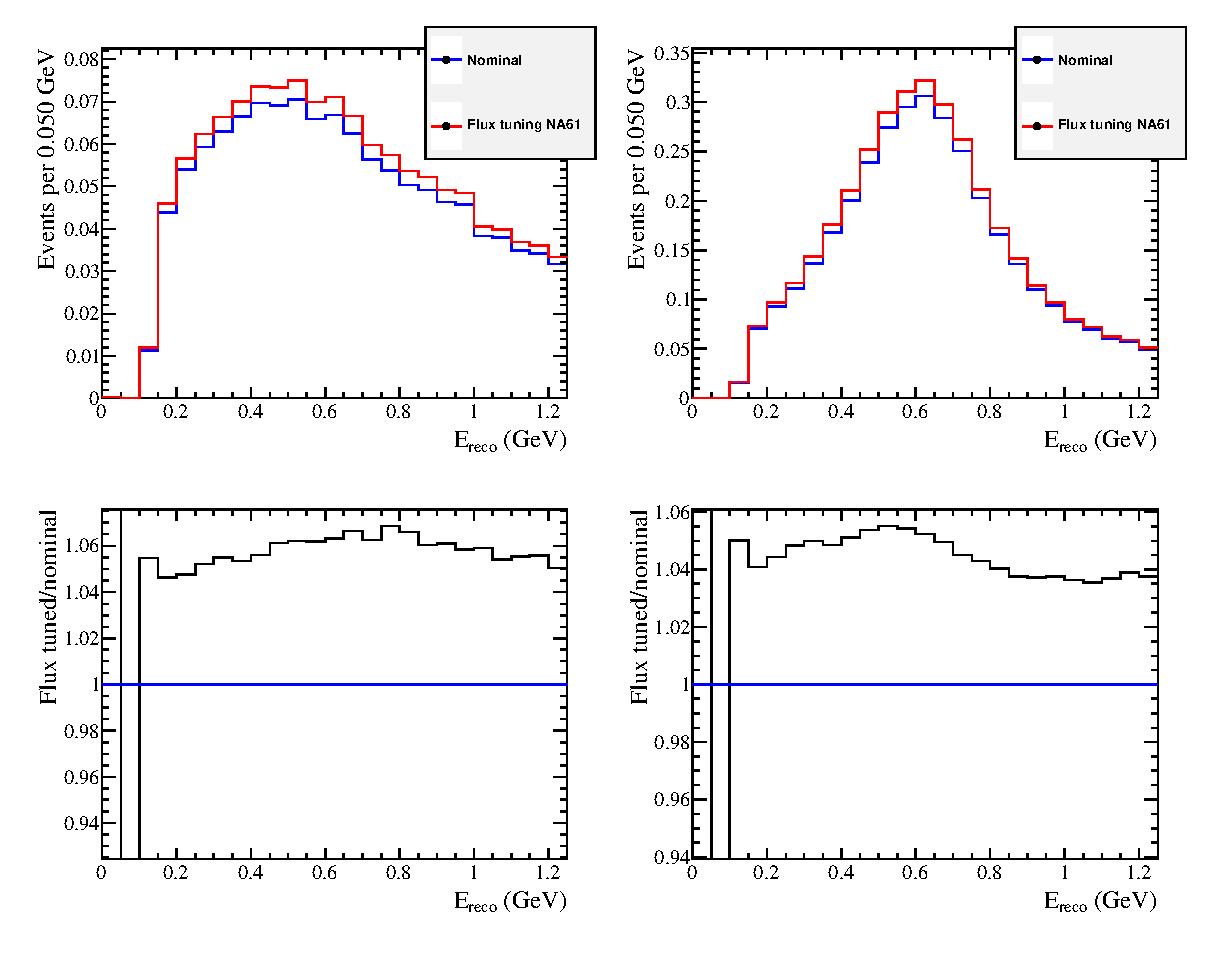
\includegraphics[width=30pc]{./nuebar_plots/spectrum_predictions/flux_tuning_effect.eps}
%\caption {
%    \huge{TO UPDATE} % caption is already ok
%{\large{SPECTRA NA61/SHINE TUNING MU-LIKE NEUTRINO MODE}}
%%Top: Reconstructed-energy spectrum of 1 $\mu$-like ring events in neutrino mode,
%%for an exposure 
%%of $6.914 \times 10^{20}$ POT %in neutrino mode
%%%and
%%%of $4.011 \times 10^{20}$ POT in antineutrino mode
%%both with and without the effect of the NA61/SHINE flux tuning of the nominal MC templates.
%%The spectra are shown both for no oscillations (left)
%%and for oscillations assuming the normal hierarchy, and the oscillation parameters shown in table~\ref{tab:osc_params_fixed_values_reactor}.
%%Bottom: Ratio of flux tuned with NA61/SHINE spectrum to the nominal MC spectrum.
%}
%\label{fig:1Rmu_spectrum_w_and_wo_na61_weights}
%\end{figure*}
%
%\begin{figure*}[htb]
%\center
%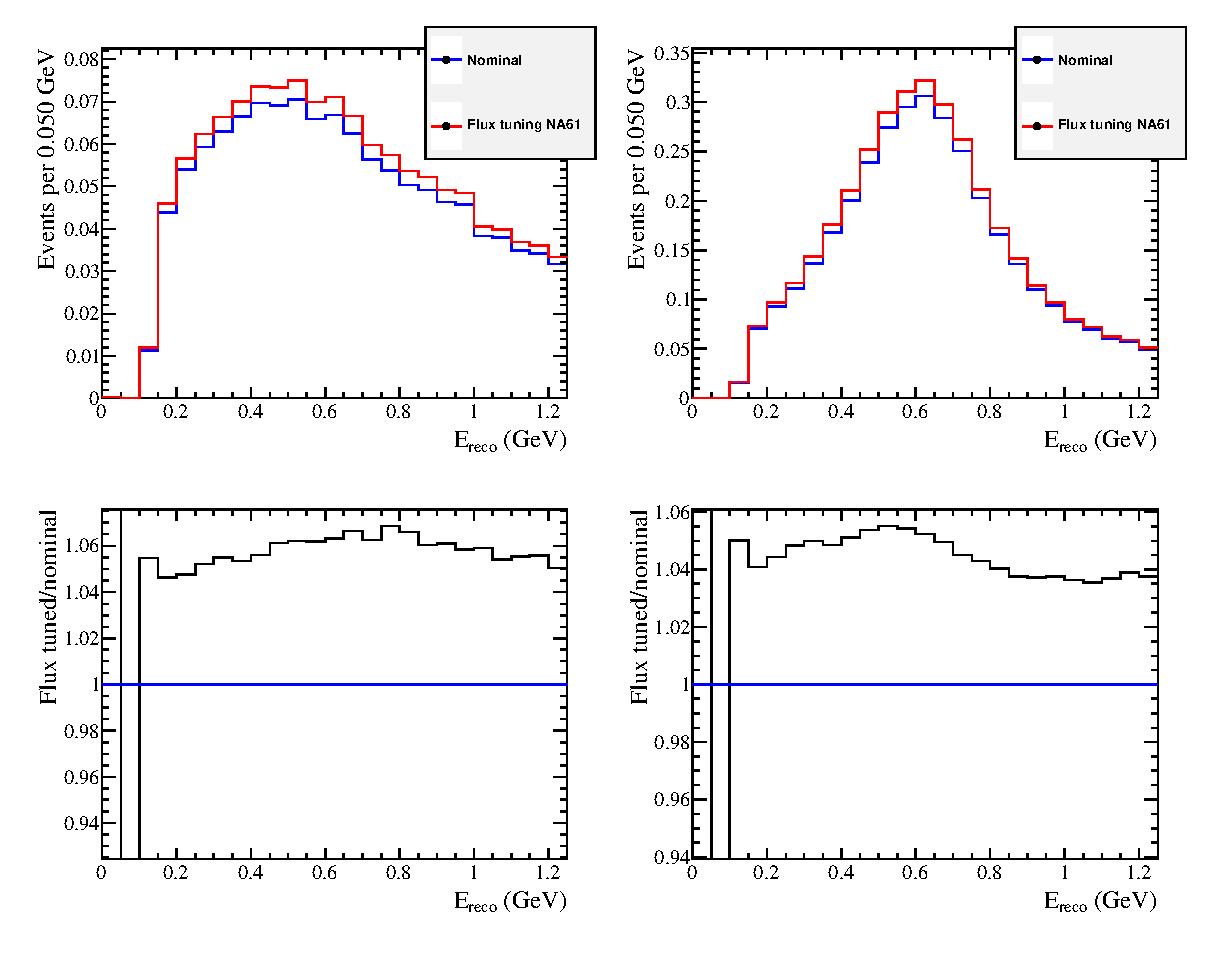
\includegraphics[width=30pc]{./nuebar_plots/spectrum_predictions/flux_tuning_effect.eps}
%\caption {
%    \huge{TO UPDATE} % caption is already ok
%{\large{SPECTRA NA61/SHINE TUNING MU-LIKE ANTINEUTRINO MODE}}
%%Top: Reconstructed-energy spectrum of 1 $\mu$-like ring events in antineutrino mode,
%%for an exposure 
%%%of $6.914 \times 10^{20}$ POT in neutrino mode
%%%and
%%of $4.011 \times 10^{20}$ POT% in antineutrino mode
%%both with and without the effect of the NA61/SHINE flux tuning of the nominal MC templates.
%%The spectra are shown both for no oscillations (left)
%%and for oscillations assuming the normal hierarchy, and the oscillation parameters shown in table~\ref{tab:osc_params_fixed_values_reactor}.
%%Bottom: Ratio of flux tuned with NA61/SHINE spectrum to the nominal MC spectrum.
%}
%\label{fig:RHC1Rmu_spectrum_w_and_wo_na61_weights}
%\end{figure*}
%
%\begin{figure*}[htb]
%\center
%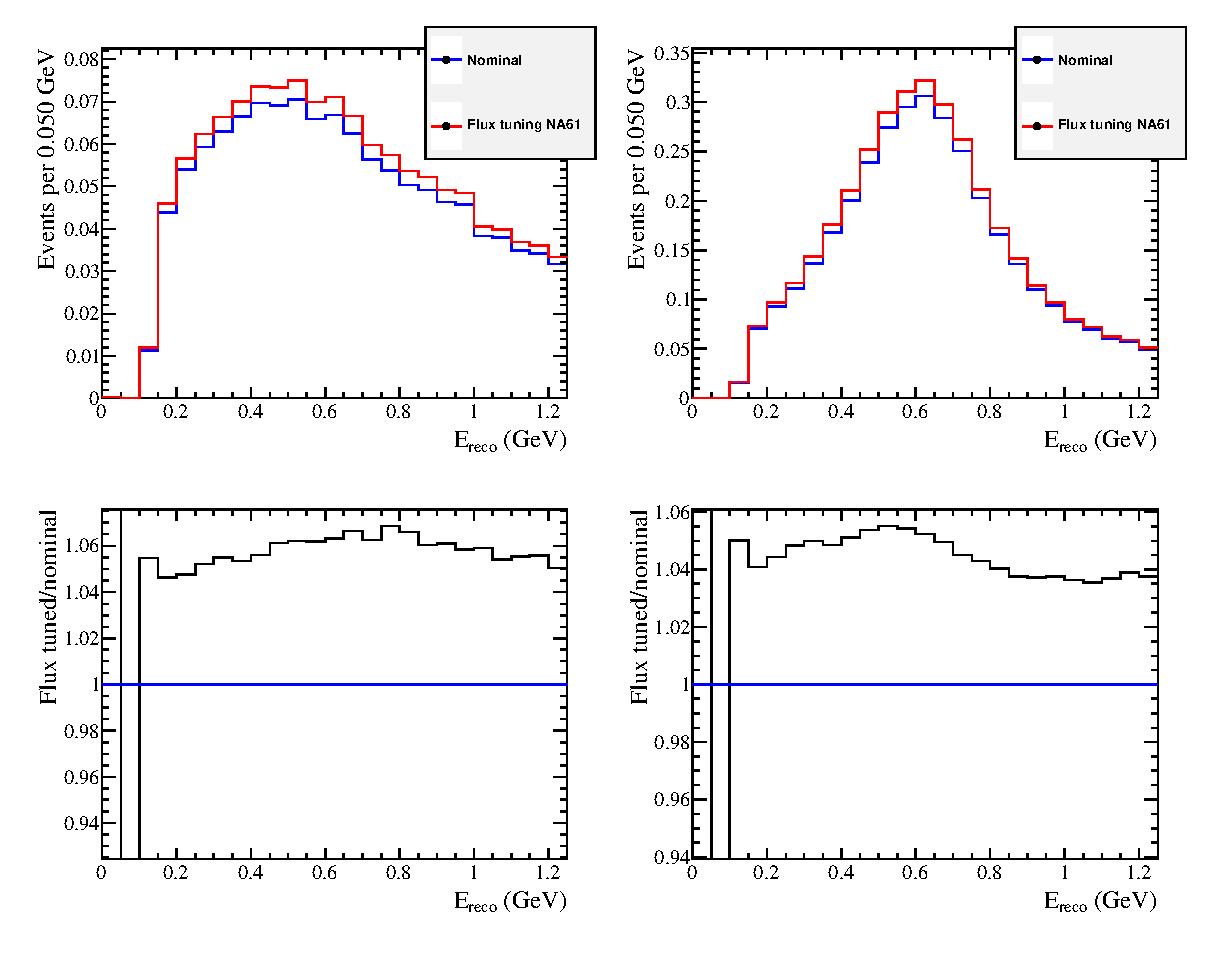
\includegraphics[width=30pc]{./nuebar_plots/spectrum_predictions/flux_tuning_effect.eps}
%\caption {
%    \huge{TO UPDATE} % caption is already ok
%{\large{SPECTRA NA61/SHINE TUNING E-LIKE NEUTRINO MODE}}
%%Top: Reconstructed-energy spectrum of 1 $e$-like ring events in neutrino mode,
%%for an exposure 
%%of $6.914 \times 10^{20}$ POT% in neutrino mode
%%%and
%%%of $4.011 \times 10^{20}$ POT in antineutrino mode
%%both with and without the effect of the NA61/SHINE flux tuning of the nominal MC templates.
%%The spectra are shown both for no oscillations (left)
%%and for oscillations assuming the normal hierarchy, and the oscillation parameters shown in table~\ref{tab:osc_params_fixed_values_reactor}.
%%Bottom: Ratio of flux tuned with NA61/SHINE spectrum to the nominal MC spectrum.
%}
%\label{fig:1Re_spectrum_w_and_wo_na61_weights}
%\end{figure*}
%
%\begin{figure*}[htb]
%\center
%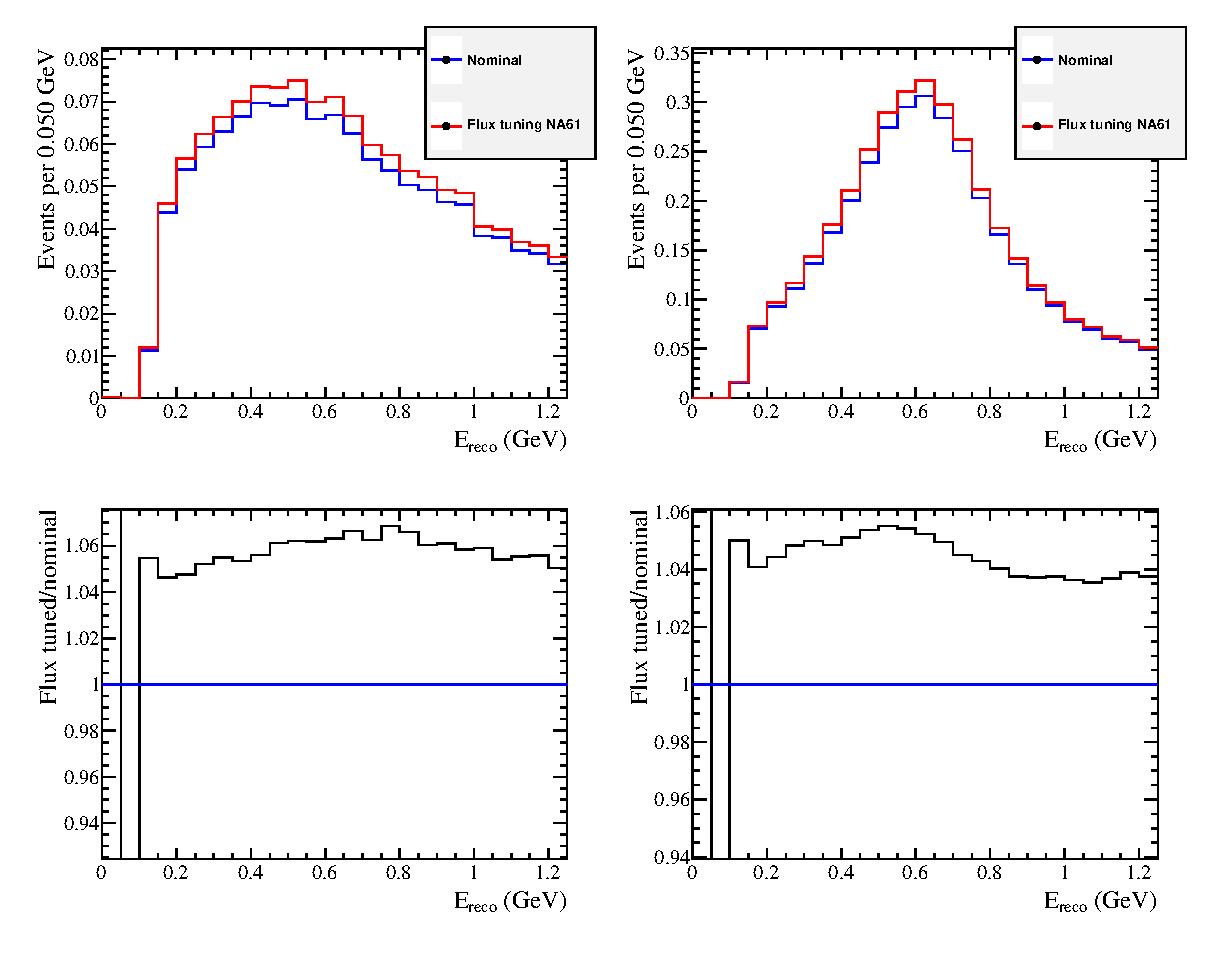
\includegraphics[width=30pc]{./nuebar_plots/spectrum_predictions/flux_tuning_effect.eps}
%\caption {
%    \huge{TO UPDATE} % caption is already ok
%{\large{SPECTRA NA61/SHINE TUNING E-LIKE ANTINEUTRINO MODE}}
%%Top: Reconstructed-energy spectrum of 1 $e$-like ring events in antineutrino mode,
%%for an exposure 
%%%of $6.914 \times 10^{20}$ POT in neutrino mode
%%%and
%%of $4.011 \times 10^{20}$ POT %in antineutrino mode
%%both with and without the effect of the NA61/SHINE flux tuning of the nominal MC templates.
%%The spectra are shown both for no oscillations (left)
%%and for oscillations assuming the normal hierarchy, and the oscillation parameters shown in table~\ref{tab:osc_params_fixed_values_reactor}.
%%Bottom: Ratio of flux tuned with NA61/SHINE spectrum to the nominal MC spectrum.
%}
%\label{fig:RHC1Re_spectrum_w_and_wo_na61_weights}
%\end{figure*}
%
%
%
%
%
%
%
%
%
%
%% Plots showing the effect of tunes on Ereco spectra w/ and w/o BANFF
%
%\begin{figure*}[htb]
%\center
%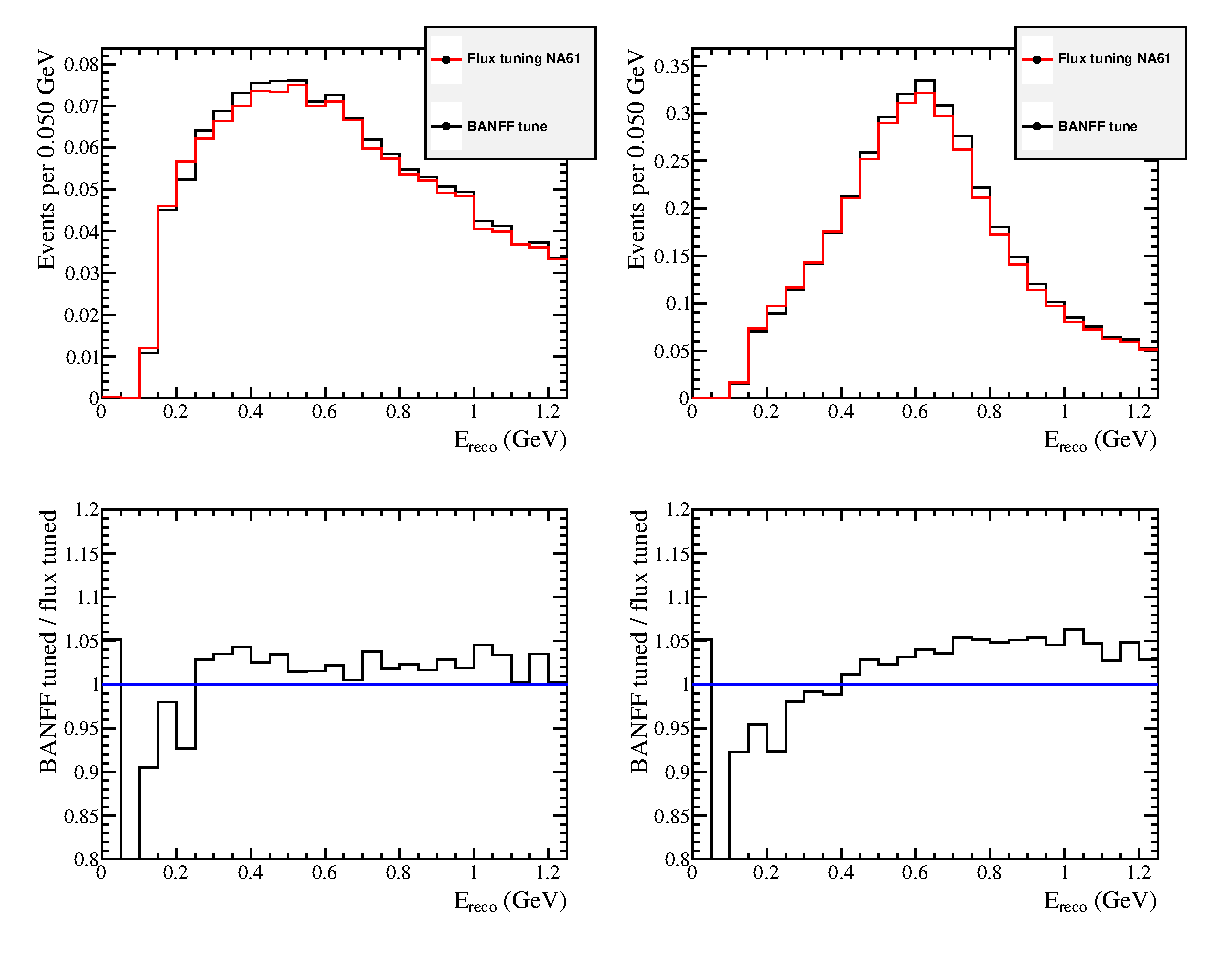
\includegraphics[width=30pc]{./nuebar_plots/spectrum_predictions/banff_tuning_effect.eps}
%\caption {
%    \huge{TO UPDATE} % caption is already ok
%{\large{SPECTRA BANFF TUNING MU-LIKE NEUTRINO MODE}}
%%Top: Reconstructed-energy spectrum of 1 $\mu$-like ring events in neutrino mode,
%%for an exposure 
%%of $6.914 \times 10^{20}$ POT % in neutrino mode
%%%and
%%%of $4.011 \times 10^{20}$ POT in antineutrino mode
%%both with and without the effect of postfit BANFF flux and cross-section tuning on the NA61/SHINE-tuned flux MC templates.
%%The spectra are shown both for no oscillations (left)
%%and for oscillations assuming the normal hierarchy, and the oscillation parameters shown in table~\ref{tab:osc_params_fixed_values_reactor}.
%%Bottom: Ratio of BANFF-tuned spectrum to the flux tuned with NA61/SHINE spectrum.
%}
%\label{fig:1Rmu_spectrum_w_and_wo_banff_weights}
%\end{figure*}
%
%\begin{figure*}[htb]
%\center
%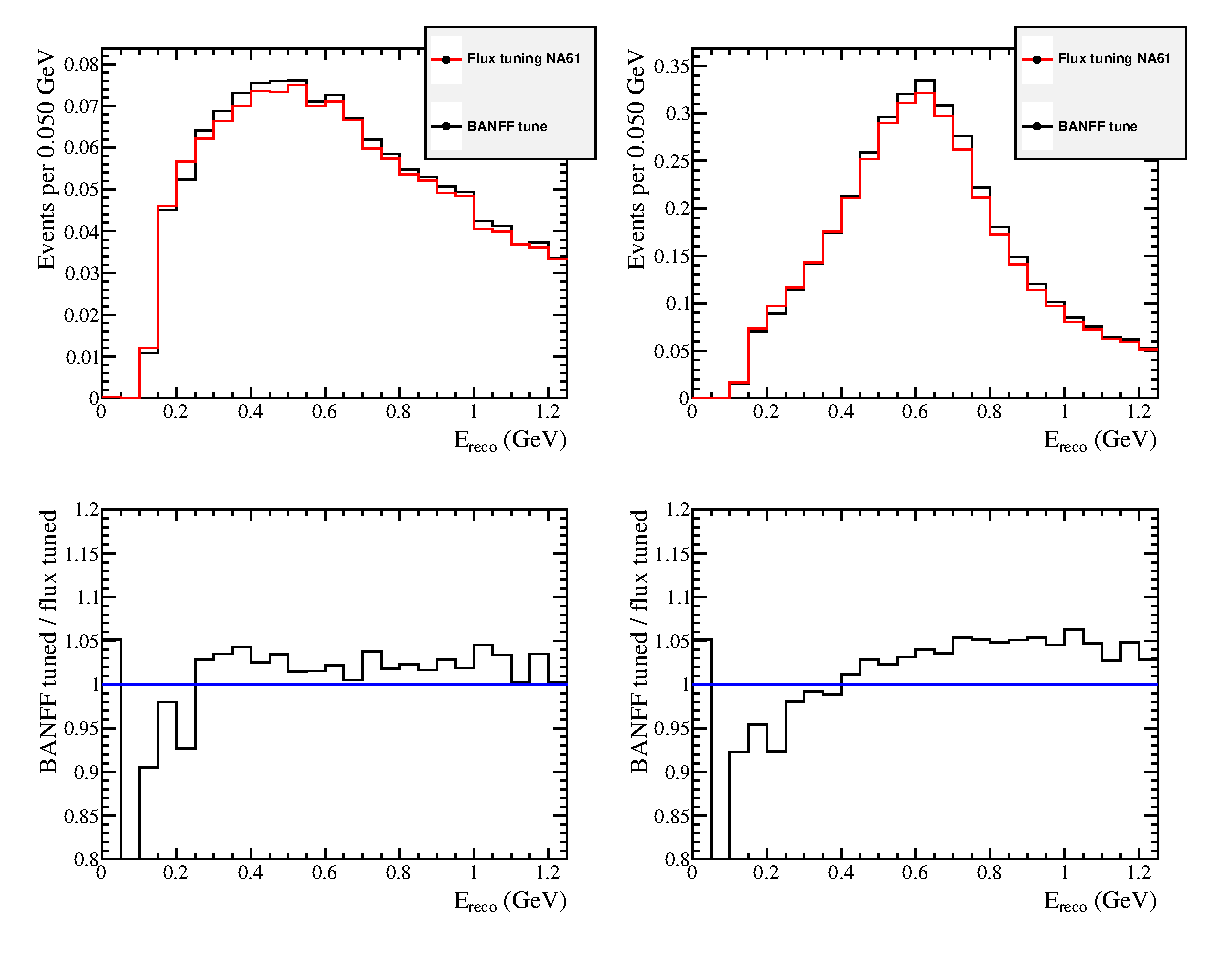
\includegraphics[width=30pc]{./nuebar_plots/spectrum_predictions/banff_tuning_effect.eps}
%\caption {
%    \huge{TO UPDATE} % caption is already ok
%{\large{SPECTRA BANFF TUNING MU-LIKE ANTINEUTRINO MODE}}
%%Top: Reconstructed-energy spectrum of 1 $\mu$-like ring events in antineutrino mode,
%%for an exposure 
%%%of $6.914 \times 10^{20}$ POT in neutrino mode
%%%and
%%of $4.011 \times 10^{20}$ POT% in antineutrino mode
%%both with and without the effect of postfit BANFF flux and cross-section tuning on the NA61/SHINE-tuned flux MC templates.
%%The spectra are shown both for no oscillations (left)
%%and for oscillations assuming the normal hierarchy, and the oscillation parameters shown in table~\ref{tab:osc_params_fixed_values_reactor}.
%%Bottom: Ratio of BANFF-tuned spectrum to the flux tuned with NA61/SHINE spectrum.
%}
%\label{fig:RHC1Rmu_spectrum_w_and_wo_banff_weights}
%\end{figure*}
%
%\begin{figure*}[htb]
%\center
%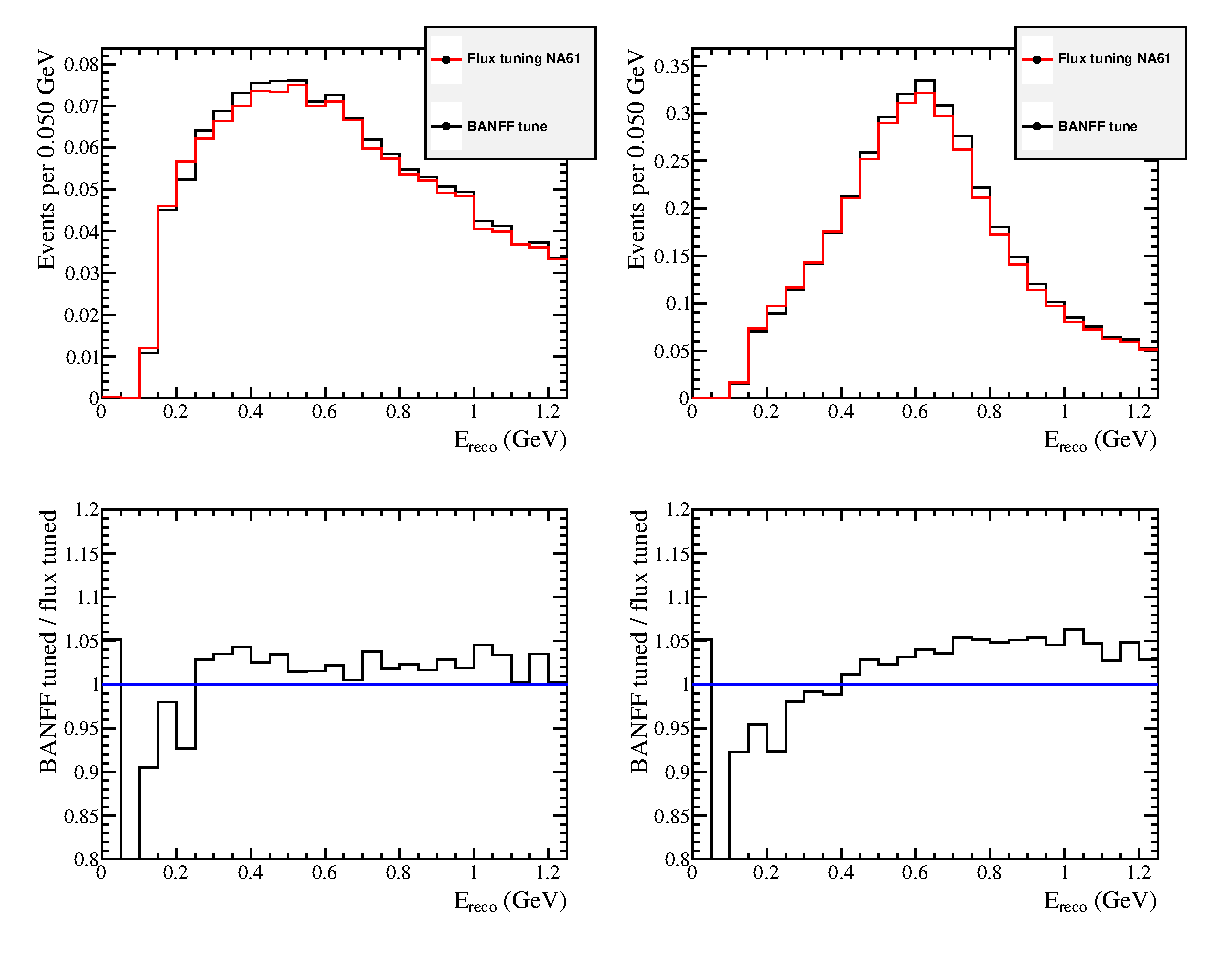
\includegraphics[width=30pc]{./nuebar_plots/spectrum_predictions/banff_tuning_effect.eps}
%\caption {
%    \huge{TO UPDATE} % caption is already ok
%{\large{SPECTRA BANFF TUNING E-LIKE NEUTRINO MODE}}
%%Top: Reconstructed-energy spectrum of 1 $e$-like ring events in neutrino mode,
%%for an exposure 
%%of $6.914 \times 10^{20}$ POT %in neutrino mode
%%%and
%%%of $4.011 \times 10^{20}$ POT in antineutrino mode
%%both with and without the effect of postfit BANFF flux and cross-section tuning on the NA61/SHINE-tuned flux MC templates.
%%The spectra are shown both for no oscillations (left)
%%and for oscillations assuming the normal hierarchy, and the oscillation parameters shown in table~\ref{tab:osc_params_fixed_values_reactor}.
%%Bottom: Ratio of BANFF-tuned spectrum to the flux tuned with NA61/SHINE spectrum.
%}
%\label{fig:1Re_spectrum_w_and_wo_banff_weights}
%\end{figure*}
%
%\begin{figure*}[htb]
%\center
%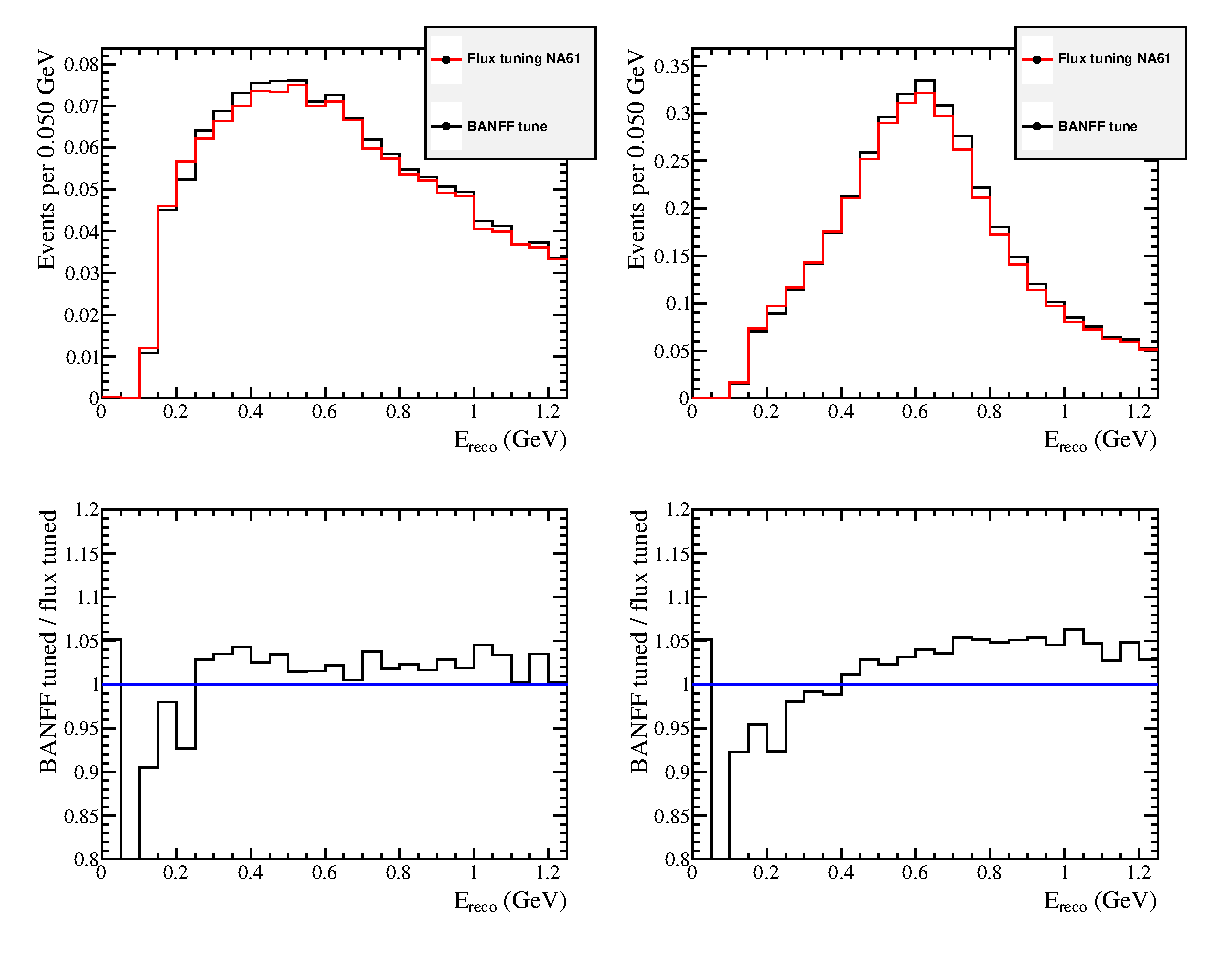
\includegraphics[width=30pc]{./nuebar_plots/spectrum_predictions/banff_tuning_effect.eps}
%\caption {
%    \huge{TO UPDATE} % caption is already ok
%{\large{SPECTRA BANFF TUNING E-LIKE ANTINEUTRINO MODE}}
%%Top: Reconstructed-energy spectrum of 1 $e$-like ring events in antineutrino mode,
%%for an exposure 
%%%of $6.914 \times 10^{20}$ POT in neutrino mode
%%%and
%%of $4.011 \times 10^{20}$ POT %in antineutrino mode
%%both with and without the effect of postfit BANFF flux and cross-section tuning on the NA61/SHINE-tuned flux MC templates.
%%The spectra are shown both for no oscillations (left)
%%and for oscillations assuming the normal hierarchy, and the oscillation parameters shown in table~\ref{tab:osc_params_fixed_values_reactor}.
%%Bottom: Ratio of BANFF-tuned spectrum to the flux tuned with NA61/SHINE spectrum.
%}
%\label{fig:RHC1Re_spectrum_w_and_wo_banff_weights}
%\end{figure*}
%
%\newpage
%\clearpage

In \cref{tab:events_1rmu_Asimov_B},
\ref{tab:events_rhc1rmu_Asimov_B} and
\ref{tab:events_1re_Asimov_B},
\ref{tab:events_rhc1re_Asimov_B} 
the total number of events expected for the Asimov data set B (see \cref{tab:osc_params_joint_asimov}) is shown.

%\newpage
\clearpage


\begin{table}
\center
\begin{tabular} { | l ||r | r | r | r | r | r | | r | }
\hline
              & $\nu_\mu$            & $\nu_e$              & $\bar{\nu_\mu}$      & $\bar{\nu_e}$        & Osc. $\nu_e$         & Osc. $\bar{\nu_e}$   & Total                \\ \hline\hline
 CCQE         & 69.747               & 0.035                & 4.335                & 0.002                & 0.151                & 0.001                & 74.270               \\ \hline
 CC1pi        & 17.206               & 0.017                & 1.572                & 0.001                & 0.049                & 0.000                & 18.845               \\ \hline
 CCcoherent   & 0.330                & 0.000                & 0.080                & 0.000                & 0.001                & 0.000                & 0.412                \\ \hline
 2p-2h          & 19.725               & 0.010                & 0.852                & 0.000                & 0.036                & 0.000                & 20.623               \\ \hline
 CCother      & 7.742                & 0.008                & 0.494                & 0.001                & 0.002                & 0.000                & 8.247                \\ \hline
 NC1pi0       & 0.537                & 0.016                & 0.017                & 0.001                & N/A                  & N/A                  & 0.572                \\ \hline
 NC1piPM      & 3.944                & 0.089                & 0.142                & 0.008                & N/A                  & N/A                  & 4.183                \\ \hline
 NCcoherent   & 0.016                & 0.000                & 0.001                & 0.000                & N/A                  & N/A                  & 0.018                \\ \hline
 NCother      & 2.993                & 0.121                & 0.165                & 0.012                & N/A                  & N/A                  & 3.290                \\ \hline
 NC1gamma     & 0.004                & 0.000                & 0.000                & 0.000                & N/A                  & N/A                  & 0.004                \\ \hline
\hline
 Total        & 122.243              & 0.297                & 7.659                & 0.025                & 0.238                & 0.002                & 130.464              \\ \hline
\end{tabular}
\caption{
%{\Huge{TO UPDATE}}
Predicted number of events in the neutrino mode $\mu$-like sample
obtained after applying the BANFF weight
for a total exposure of \TotalPotNu{} POT.
The Asimov data set B in \cref{tab:osc_params_joint_asimov} is used.
}
\label{tab:events_1rmu_Asimov_B}
\end{table}




\begin{table}
\center
\begin{tabular} { | l ||r | r | r | r | r | r | | r | }
\hline
             & $\nu_\mu$            & $\nu_e$              & $\bar{\nu_\mu}$      & $\bar{\nu_e}$        & Osc. $\nu_e$         & Osc. $\bar{\nu_e}$   & Total                \\ \hline\hline
 CCQE         & 7.088                & 0.004                & 13.306               & 0.005                & 0.004                & 0.016                & 20.422               \\ \hline
 CC1pi        & 2.718                & 0.003                & 3.066                & 0.002                & 0.002                & 0.003                & 5.794                \\ \hline
 CCcoherent   & 0.054                & 0.000                & 0.173                & 0.000                & 0.000                & 0.000                & 0.228                \\ \hline
 2p-2h          & 2.525                & 0.001                & 2.118                & 0.001                & 0.001                & 0.002                & 4.649                \\ \hline
 CCother      & 1.282                & 0.001                & 0.886                & 0.000                & 0.000                & 0.000                & 2.170                \\ \hline
 NC1pi0       & 0.060                & 0.002                & 0.050                & 0.001                & N/A                  & N/A                  & 0.114                \\ \hline
 NC1piPM      & 0.378                & 0.015                & 0.380                & 0.010                & N/A                  & N/A                  & 0.784                \\ \hline
 NCcoherent   & 0.001                & 0.000                & 0.006                & 0.000                & N/A                  & N/A                  & 0.008                \\ \hline
 NCother      & 0.530                & 0.025                & 0.296                & 0.012                & N/A                  & N/A                  & 0.862                \\ \hline
 NC1gamma     & 0.000                & 0.000                & 0.000                & 0.000                & N/A                  & N/A                  & 0.000                \\ \hline
\hline
 Total        & 14.637               & 0.051                & 20.282               & 0.032                & 0.008                & 0.022                & 35.032               \\ \hline

\end{tabular}
\caption{
%{\Huge{TO UPDATE}}
Predicted number of events in the antineutrino mode $\mu$-like sample
obtained after applying the BANFF weight
for a total exposure of \TotalPotNuBar{} POT.
The Asimov data set B in \cref{tab:osc_params_joint_asimov} is used.
}
\label{tab:events_rhc1rmu_Asimov_B}
\end{table}




\begin{table}
\center
\begin{tabular} { | l ||r | r | r | r | r | r | | r | }
\hline
              & $\nu_\mu$            & $\nu_e$              & $\bar{\nu_\mu}$      & $\bar{\nu_e}$        & Osc. $\nu_e$         & Osc. $\bar{\nu_e}$   & Total                \\ \hline\hline
 CCQE         & 0.062                & 2.129                & 0.001                & 0.088                & 10.811               & 0.121                & 13.211               \\ \hline
 CC1pi        & 0.017                & 0.348                & 0.000                & 0.027                & 1.236                & 0.020                & 1.648                \\ \hline
 CCcoherent   & 0.000                & 0.002                & 0.000                & 0.002                & 0.011                & 0.002                & 0.017                \\ \hline
 2p-2h          & 0.009                & 0.710                & 0.000                & 0.022                & 2.750                & 0.022                & 3.513                \\ \hline
 CCother      & 0.001                & 0.045                & 0.000                & 0.003                & 0.025                & 0.001                & 0.076                \\ \hline
 NC1pi0       & 0.524                & 0.012                & 0.017                & 0.001                & N/A                  & N/A                  & 0.553                \\ \hline
 NC1piPM      & 0.099                & 0.002                & 0.003                & 0.000                & N/A                  & N/A                  & 0.105                \\ \hline
 NCcoherent   & 0.174                & 0.004                & 0.018                & 0.001                & N/A                  & N/A                  & 0.197                \\ \hline
 NCother      & 0.126                & 0.005                & 0.008                & 0.001                & N/A                  & N/A                  & 0.139                \\ \hline
 NC1gamma     & 0.464                & 0.007                & 0.021                & 0.001                & N/A                  & N/A                  & 0.494                \\ \hline
\hline
 Total        & 1.476                & 3.264                & 0.069                & 0.145                & 14.833               & 0.167                & 19.954               \\ \hline

\end{tabular}
\caption{
%{\Huge{TO UPDATE}}
Predicted number of events in the neutrino mode $e$-like sample
obtained after applying the BANFF weight
for a total exposure of \TotalPotNu{} POT.
The Asimov data set B in \cref{tab:osc_params_joint_asimov} is used.
}
\label{tab:events_1re_Asimov_B}
\end{table}




\begin{table}
\center
\begin{tabular} { | l ||r | r | r | r | r | r | | r | }
\hline
              & $\nu_\mu$            & $\nu_e$              & $\bar{\nu_\mu}$      & $\bar{\nu_e}$        & Osc. $\nu_e$         & Osc. $\bar{\nu_e}$   & Total                \\ \hline\hline
 CCQE         & 0.002                & 0.189                & 0.003                & 0.339                & 0.269                & 1.376                & 2.178                \\ \hline
 CC1pi        & 0.002                & 0.040                & 0.001                & 0.060                & 0.045                & 0.163                & 0.312                \\ \hline
 CCcoherent   & 0.000                & 0.000                & 0.000                & 0.006                & 0.000                & 0.022                & 0.029                \\ \hline
 2p-2h          & 0.001                & 0.069                & 0.000                & 0.063                & 0.087                & 0.219                & 0.439                \\ \hline
 CCother      & 0.001                & 0.008                & 0.000                & 0.004                & 0.003                & 0.003                & 0.019                \\ \hline
 NC1pi0       & 0.045                & 0.002                & 0.049                & 0.001                & N/A                  & N/A                  & 0.098                \\ \hline
 NC1piPM      & 0.011                & 0.000                & 0.008                & 0.000                & N/A                  & N/A                  & 0.020                \\ \hline
 NCcoherent   & 0.021                & 0.001                & 0.081                & 0.001                & N/A                  & N/A                  & 0.103                \\ \hline
 NCother      & 0.022                & 0.001                & 0.012                & 0.000                & N/A                  & N/A                  & 0.035                \\ \hline
 NC1gamma     & 0.037                & 0.002                & 0.081                & 0.002                & N/A                  & N/A                  & 0.121                \\ \hline
\hline
 Total        & 0.142                & 0.313                & 0.235                & 0.478                & 0.404                & 1.783                & 3.355                \\ \hline

\end{tabular}
\caption{
%{\Huge{TO UPDATE}}
Predicted number of events in the antineutrino mode $\mu$-like sample
obtained after applying the BANFF weight
for a total exposure of \TotalPotNuBar{} POT.
The Asimov data set B in \cref{tab:osc_params_joint_asimov} is used.
}
\label{tab:events_rhc1re_Asimov_B}
\end{table}





\newpage
\clearpage

In \cref{tab:events_1rmu_NoOsc},
\ref{tab:events_rhc1rmu_NoOsc} and
\ref{tab:events_1re_NoOsc},
\ref{tab:events_rhc1re_NoOsc}
the total number of unoscillated events is shown.
 

\begin{table}
\center
\begin{tabular} { | l ||r | r | r | r | r | r | | r | }
\hline
              & $\nu_\mu$            & $\nu_e$              & $\bar{\nu_\mu}$      & $\bar{\nu_e}$        & Osc. $\nu_e$         & Osc. $\bar{\nu_e}$   & Total                \\ \hline\hline
 CCQE         & 338.683              & 0.037                & 8.672                & 0.002                & 0.000                & 0.000                & 347.394              \\ \hline
 CC1pi        & 39.668               & 0.018                & 2.276                & 0.001                & 0.000                & 0.000                & 41.963               \\ \hline
 CCcoherent   & 0.678                & 0.000                & 0.136                & 0.000                & 0.000                & 0.000                & 0.815                \\ \hline
 2p-2h          & 74.638               & 0.011                & 1.548                & 0.000                & 0.000                & 0.000                & 76.198               \\ \hline
 CCother      & 8.732                & 0.009                & 0.560                & 0.001                & 0.000                & 0.000                & 9.301                \\ \hline
 NC1pi0       & 0.537                & 0.016                & 0.017                & 0.001                & N/A                  & N/A                  & 0.572                \\ \hline
 NC1piPM      & 3.944                & 0.089                & 0.142                & 0.008                & N/A                  & N/A                  & 4.183                \\ \hline
 NCcoherent   & 0.016                & 0.000                & 0.001                & 0.000                & N/A                  & N/A                  & 0.018                \\ \hline
 NCother      & 2.993                & 0.121                & 0.165                & 0.012                & N/A                  & N/A                  & 3.290                \\ \hline
 NC1gamma     & 0.004                & 0.000                & 0.000                & 0.000                & N/A                  & N/A                  & 0.004                \\ \hline
\hline
 Total        & 469.893              & 0.301                & 13.518               & 0.025                & 0.000                & 0.000                & 483.737              \\ \hline
\end{tabular}
\caption{
%{\Huge{TO UPDATE}}
Predicted number of events in the neutrino mode $\mu$-like sample
obtained after applying the BANFF weight
for a total exposure of \TotalPotNu{} POT.
Oscillations are not applied.
}
\label{tab:events_1rmu_NoOsc}
\end{table}




\begin{table}
\center
\begin{tabular} { | l ||r | r | r | r | r | r | | r | }
\hline
              & $\nu_\mu$            & $\nu_e$              & $\bar{\nu_\mu}$      & $\bar{\nu_e}$        & Osc. $\nu_e$         & Osc. $\bar{\nu_e}$   & Total                \\ \hline\hline
 CCQE         & 15.420               & 0.004                & 55.525               & 0.005                & 0.000                & 0.000                & 70.954               \\ \hline
 CC1pi        & 4.071                & 0.003                & 6.536                & 0.002                & 0.000                & 0.000                & 10.611               \\ \hline
 CCcoherent   & 0.074                & 0.000                & 0.612                & 0.000                & 0.000                & 0.000                & 0.687                \\ \hline
 2p-2h          & 4.721                & 0.001                & 7.811                & 0.001                & 0.000                & 0.000                & 12.534               \\ \hline
 CCother      & 1.457                & 0.001                & 1.008                & 0.000                & 0.000                & 0.000                & 2.467                \\ \hline
 NC1pi0       & 0.060                & 0.002                & 0.050                & 0.001                & N/A                  & N/A                  & 0.114                \\ \hline
 NC1piPM      & 0.378                & 0.015                & 0.380                & 0.010                & N/A                  & N/A                  & 0.784                \\ \hline
 NCcoherent   & 0.001                & 0.000                & 0.006                & 0.000                & N/A                  & N/A                  & 0.008                \\ \hline
 NCother      & 0.530                & 0.025                & 0.296                & 0.012                & N/A                  & N/A                  & 0.862                \\ \hline
 NC1gamma     & 0.000                & 0.000                & 0.000                & 0.000                & N/A                  & N/A                  & 0.000                \\ \hline
\hline
 Total        & 26.713               & 0.052                & 72.225               & 0.032                & 0.000                & 0.000                & 99.021               \\ \hline

\end{tabular}
\caption{
%{\Huge{TO UPDATE}}
Predicted number of events in the antineutrino mode $\mu$-like sample
obtained after applying the BANFF weight
for a total exposure of \TotalPotNuBar{} POT.
Oscillations are not applied.
}
\label{tab:events_rhc1rmu_NoOsc}
\end{table}




\begin{table}
\center
\begin{tabular} { | l ||r | r | r | r | r | r | | r | }
\hline
               & $\nu_\mu$            & $\nu_e$              & $\bar{\nu_\mu}$      & $\bar{\nu_e}$        & Osc. $\nu_e$         & Osc. $\bar{\nu_e}$   & Total                \\ \hline\hline
 CCQE         & 0.413                & 2.294                & 0.002                & 0.094                & 0.000                & 0.000                & 2.803                \\ \hline
 CC1pi        & 0.069                & 0.371                & 0.001                & 0.028                & 0.000                & 0.000                & 0.469                \\ \hline
 CCcoherent   & 0.002                & 0.003                & 0.000                & 0.002                & 0.000                & 0.000                & 0.006                \\ \hline
 2p-2h          & 0.095                & 0.759                & 0.000                & 0.023                & 0.000                & 0.000                & 0.878                \\ \hline
 CCother      & 0.004                & 0.046                & 0.000                & 0.003                & 0.000                & 0.000                & 0.054                \\ \hline
 NC1pi0       & 0.524                & 0.012                & 0.017                & 0.001                & N/A                  & N/A                  & 0.553                \\ \hline
 NC1piPM      & 0.099                & 0.002                & 0.003                & 0.000                & N/A                  & N/A                  & 0.105                \\ \hline
 NCcoherent   & 0.174                & 0.004                & 0.018                & 0.001                & N/A                  & N/A                  & 0.197                \\ \hline
 NCother      & 0.126                & 0.005                & 0.008                & 0.001                & N/A                  & N/A                  & 0.139                \\ \hline
 NC1gamma     & 0.464                & 0.007                & 0.021                & 0.001                & N/A                  & N/A                  & 0.494                \\ \hline
\hline
 Total        & 1.970                & 3.504                & 0.071                & 0.154                & 0.000                & 0.000                & 5.698                \\ \hline

\end{tabular}
\caption{
%{\Huge{TO UPDATE}}
Predicted number of events in the neutrino mode $e$-like sample
obtained after applying the BANFF weight
for a total exposure of \TotalPotNu{} POT.
Oscillations are not applied.
}
\label{tab:events_1re_NoOsc}
\end{table}




\begin{table}
\center
\begin{tabular} { | l ||r | r | r | r | r | r | | r | }
\hline
              & $\nu_\mu$            & $\nu_e$              & $\bar{\nu_\mu}$      & $\bar{\nu_e}$        & Osc. $\nu_e$         & Osc. $\bar{\nu_e}$   & Total                \\ \hline\hline
 CCQE         & 0.012                & 0.203                & 0.018                & 0.361                & 0.000                & 0.000                & 0.593                \\ \hline
 CC1pi        & 0.004                & 0.043                & 0.003                & 0.064                & 0.000                & 0.000                & 0.114                \\ \hline
 CCcoherent   & 0.000                & 0.000                & 0.000                & 0.006                & 0.000                & 0.000                & 0.007                \\ \hline
 2p-2h          & 0.003                & 0.074                & 0.003                & 0.067                & 0.000                & 0.000                & 0.147                \\ \hline
 CCother      & 0.001                & 0.009                & 0.000                & 0.004                & 0.000                & 0.000                & 0.015                \\ \hline
 NC1pi0       & 0.045                & 0.002                & 0.049                & 0.001                & N/A                  & N/A                  & 0.098                \\ \hline
 NC1piPM      & 0.011                & 0.000                & 0.008                & 0.000                & N/A                  & N/A                  & 0.020                \\ \hline
 NCcoherent   & 0.021                & 0.001                & 0.081                & 0.001                & N/A                  & N/A                  & 0.103                \\ \hline
 NCother      & 0.022                & 0.001                & 0.012                & 0.000                & N/A                  & N/A                  & 0.035                \\ \hline
 NC1gamma     & 0.037                & 0.002                & 0.081                & 0.002                & N/A                  & N/A                  & 0.121                \\ \hline
\hline
 Total        & 0.156                & 0.334                & 0.255                & 0.507                & 0.000                & 0.000                & 1.253                \\ \hline

\end{tabular}
\caption{
%{\Huge{TO UPDATE}}
Predicted number of events in the antineutrino mode $e$-like sample
obtained after applying the BANFF weight
for a total exposure of \TotalPotNuBar{} POT.
Oscillations are not applied.
}
\label{tab:events_rhc1re_NoOsc}
\end{table}





\clearpage





